\documentclass{beamer}
\usepackage{amsthm}
\usepackage{times}
\usepackage{graphicx}
\usefonttheme{professionalfonts}
\usetheme{Boadilla}
%\usecolortheme{sidebartab}
\title{Interbrain data analysis}
%\subtitle{L'equazione di Fisher}
\author[F. Bernardi]{\textbf{Fabrizio Bernardi}} \medskip
%\titlegraphic{
\includegraphics[scale=.1]{Logo_Politecnico_Milano.jpg}}
%\titlegraphic{
\includegraphics[scale=.3]{Logo_IIT.png}}





\date[09/12/2021]{09/12/2021}


\begin{document}
		\begin{frame}
	\maketitle
	
	\begin{minipage}{\linewidth}
		\centering
		\begin{minipage}{0.45\linewidth}
			\begin{figure}[H]
				
\includegraphics[width=\linewidth]{Logo_IIT.png}
				
			\end{figure}
		\end{minipage}
		\hspace{0.05\linewidth}
		\begin{minipage}{0.45\linewidth}
			\begin{figure}[H]
				
\includegraphics[width=\linewidth]{Logo_Politecnico_Milano.jpg}
				
			\end{figure}
		\end{minipage}
	\end{minipage}
\end{frame}

\begin{frame}
\frametitle{Average $L^2$ errors with neutral observer}


\begin{figure}[H]
	\begin{center}
		\hspace*{-1.7cm}
		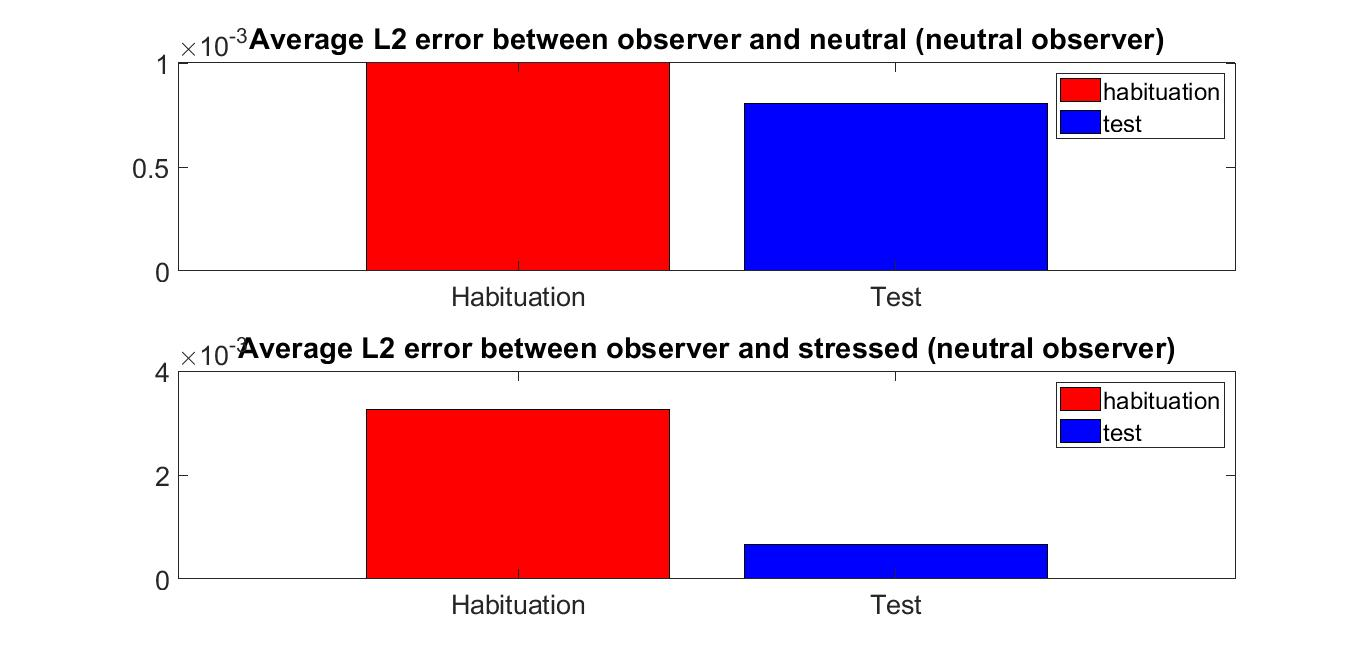
\includegraphics[scale=.32]{avg_L2.jpg} 
	\end{center}  
	
	
\end{figure}



\end{frame}

\begin{frame}
\frametitle{Average $L^2$ errors with stressed observer}


\begin{figure}[H]
\begin{center}
	\hspace*{-1.7cm}
	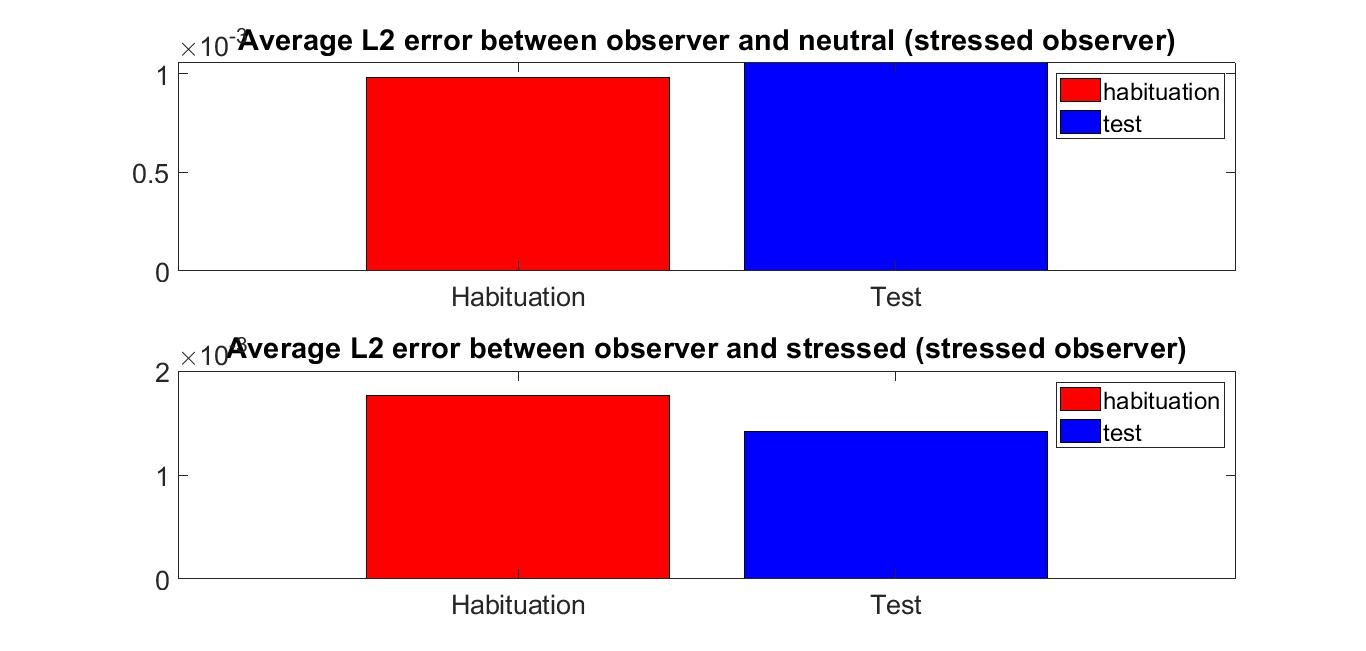
\includegraphics[scale=.32]{avg_L22.jpg} 
\end{center}  


\end{figure}



\end{frame}

\begin{frame}
\frametitle{ Average correlation between observer and stressed with neutral observer}



\begin{figure}[H]
	\begin{center}
		\hspace*{-1.7cm}
		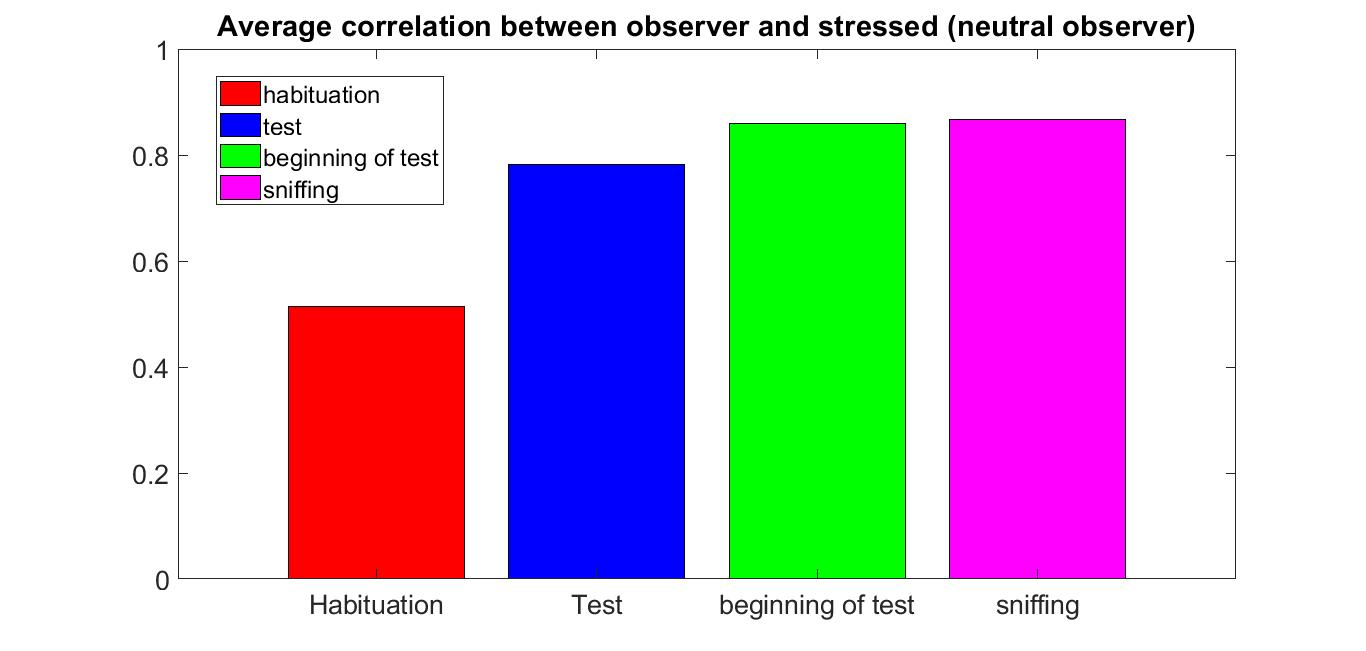
\includegraphics[scale=.32]{avg_corr_stress.jpg} 
	\end{center}  
	
	
\end{figure}

\end{frame}

\begin{frame}
\frametitle{ Average correlation between observer and neutral with neutral observer}



\begin{figure}[H]
	\begin{center}
		\hspace*{-1.7cm}
		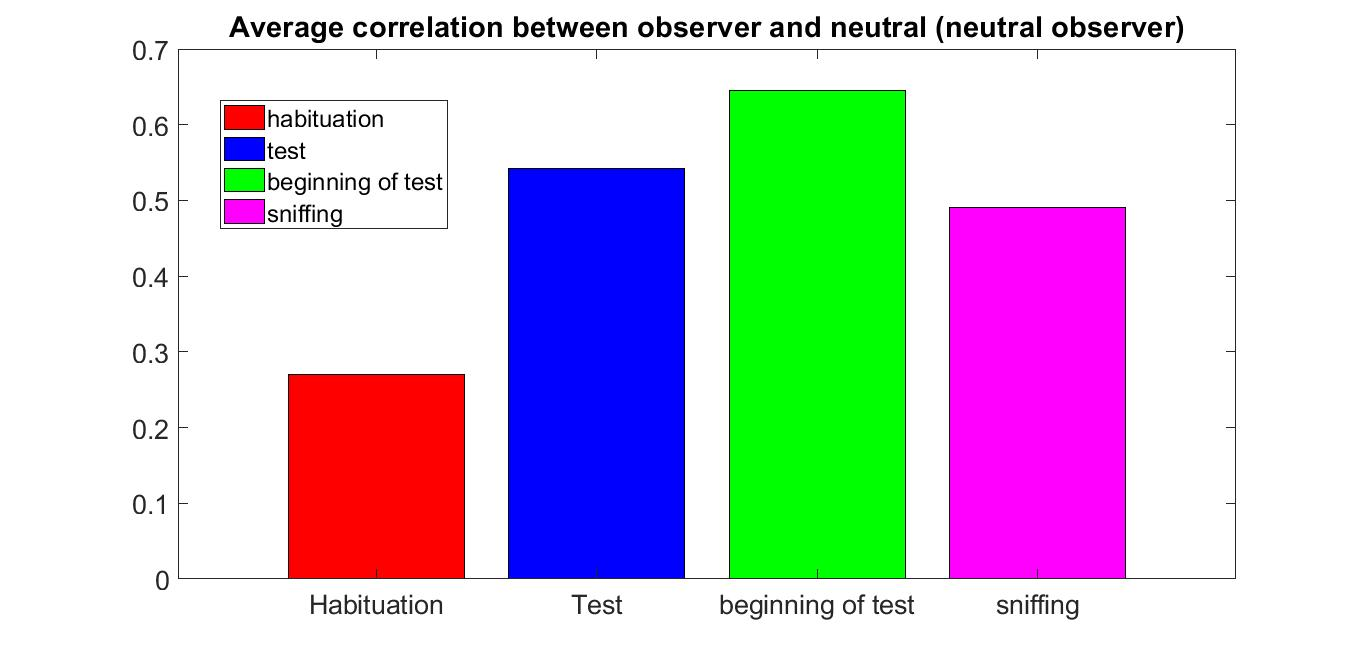
\includegraphics[scale=.32]{avg_corr_neut.jpg} 
	\end{center}  
	
	
\end{figure}

\end{frame}

\begin{frame}
\frametitle{ Average correlation between observer and stressed with stressed observer}



\begin{figure}[H]
\begin{center}
	\hspace*{-1.7cm}
	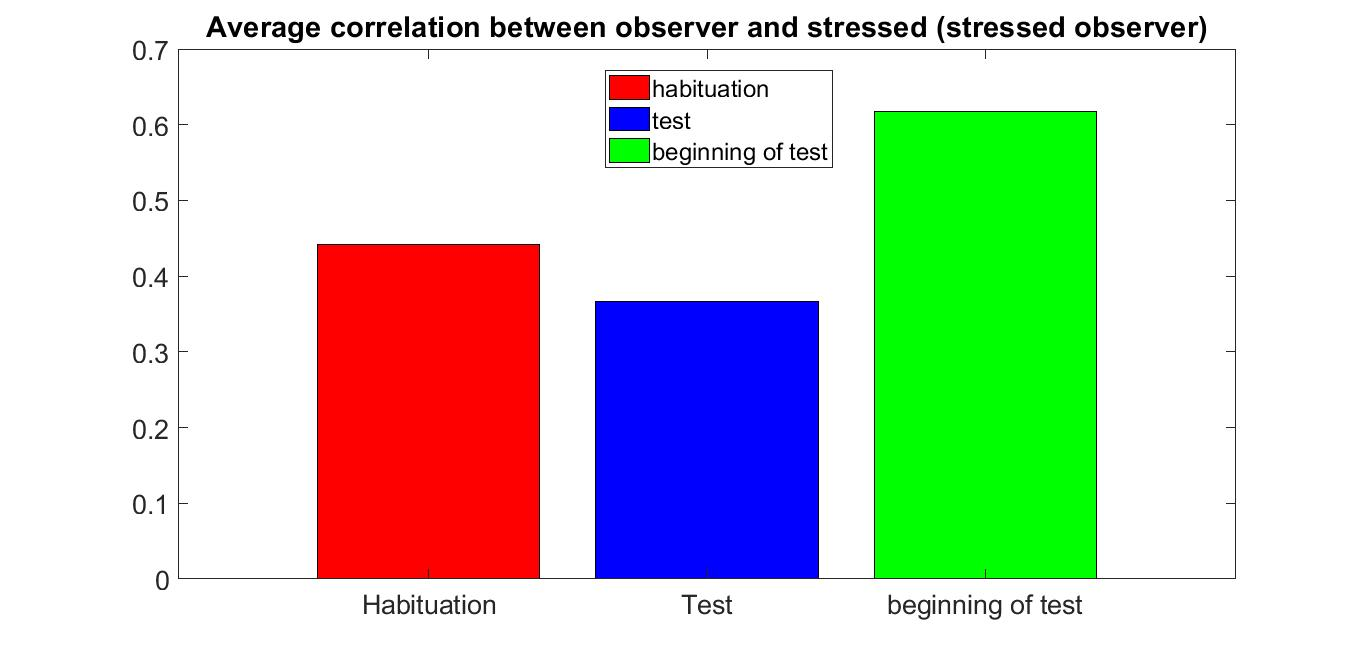
\includegraphics[scale=.32]{avg_corr_stress2.jpg} 
\end{center}  


\end{figure}

\end{frame}



\begin{frame}
\frametitle{ Average correlation between observer and neutral with stressed observer}



\begin{figure}[H]
\begin{center}
\hspace*{-1.7cm}
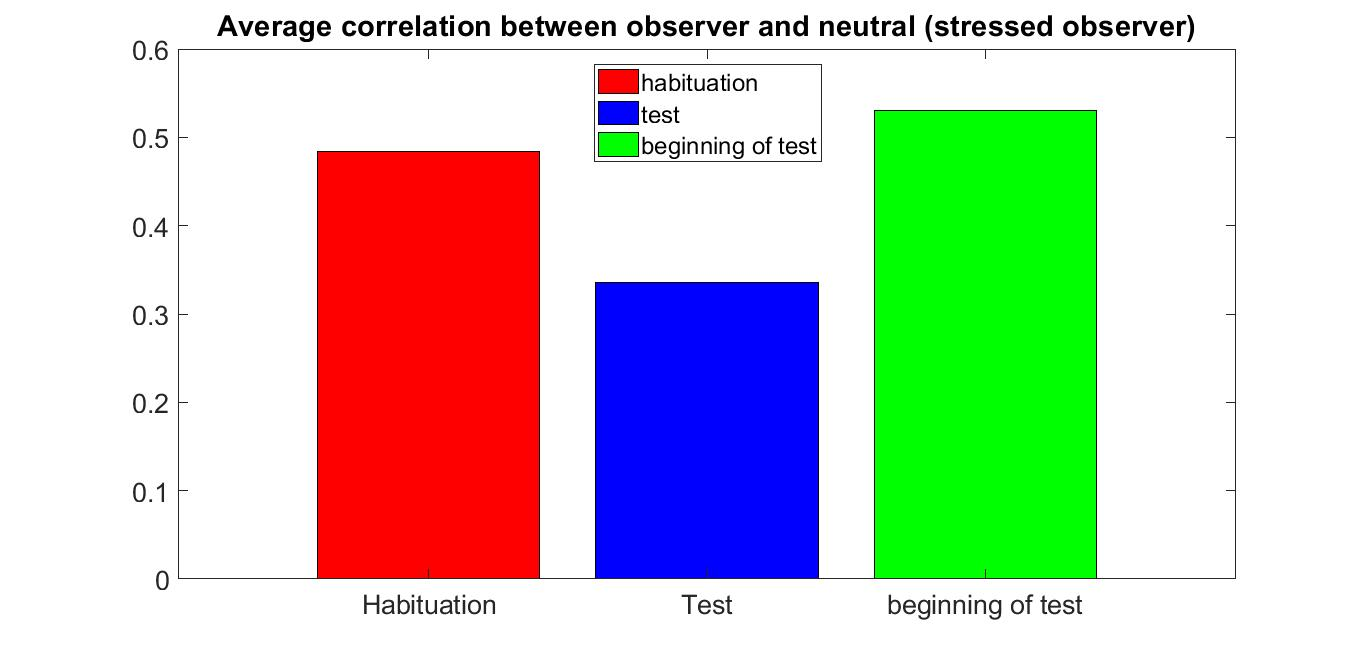
\includegraphics[scale=.32]{avg_corr_neut2.jpg} 
\end{center}  


\end{figure}

\end{frame}

\begin{frame}
\frametitle{ Stressed mice activity in all datasets}



\begin{figure}[H]
	\begin{center}
		\hspace*{-2.1 cm}
		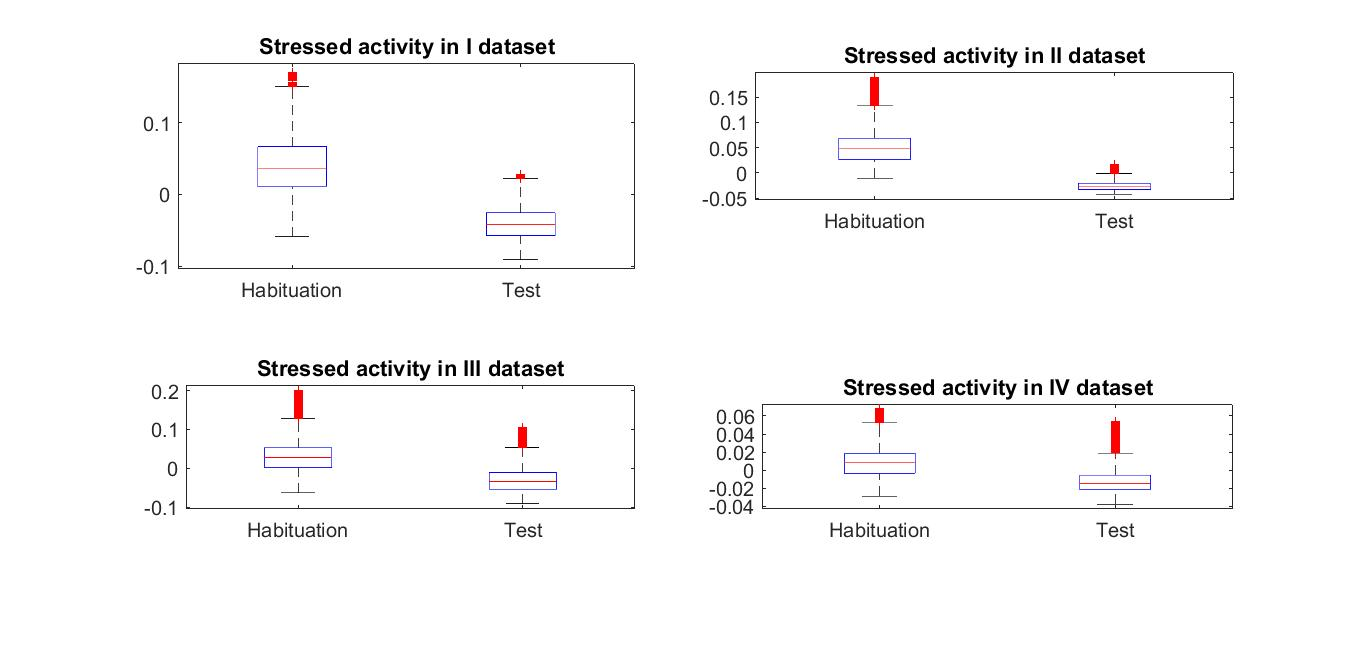
\includegraphics[scale=.33]{stressed_boxplot.jpg} 
	\end{center}  
	
	
\end{figure}

\end{frame}

\begin{frame}
\frametitle{ Average stressed mice activity}



\begin{figure}[H]
	\begin{center}
		\hspace*{-1.3cm}
		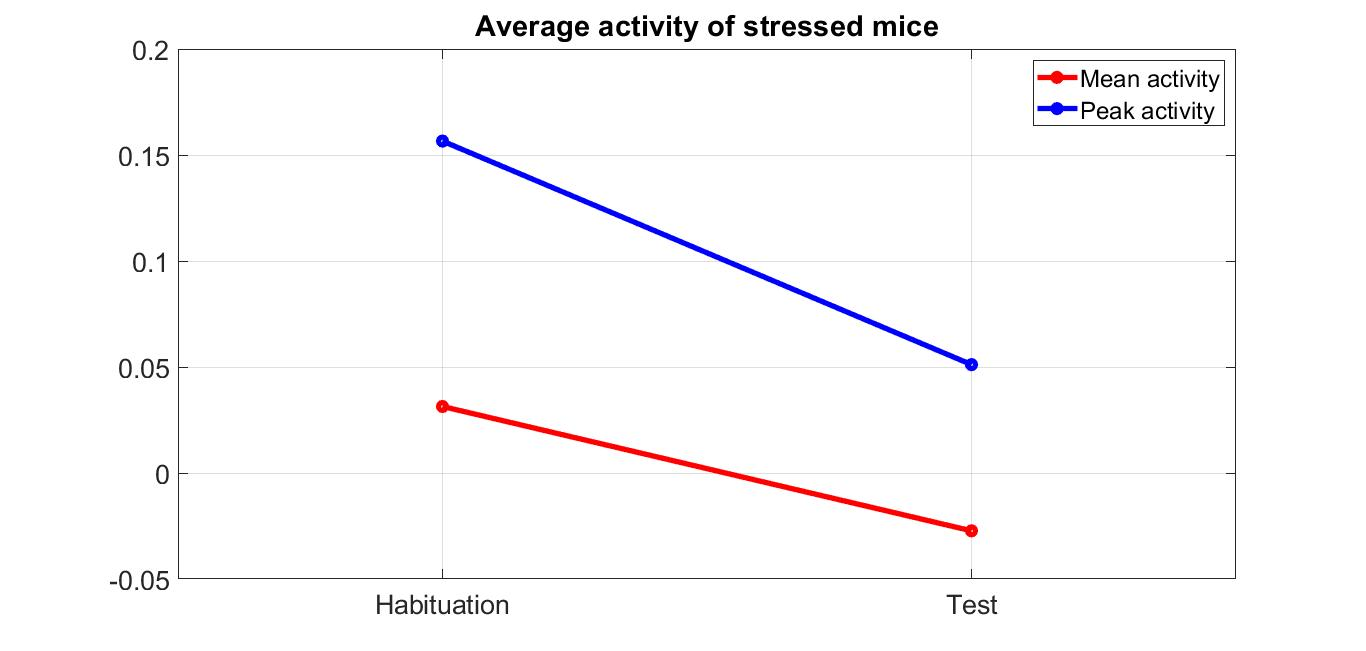
\includegraphics[scale=.30]{stressed_avg.jpg} 
	\end{center}  
	
	
\end{figure}

\end{frame}


\begin{frame}
\frametitle{Pattern recognition in activity peaks }


The pattern recognition analysis follows the steps: \vspace{1.4 cm}

\begin{enumerate}
	
	\item Detect peak activity through appropriate algorithms  \vspace{0.7 cm}
	
	\item Partition the overall time interval in windows of a fixed length and associate the presence of an event or not for every time window  \vspace{0.7 cm}
	
	\item Confront different signals to look for simultaneous events
	
\end{enumerate}
\end{frame}


\begin{frame}
\frametitle{Activity detection: MAD algorithm}

\begin{figure}[H]
	\begin{center}
		\hspace*{-1.3cm}
		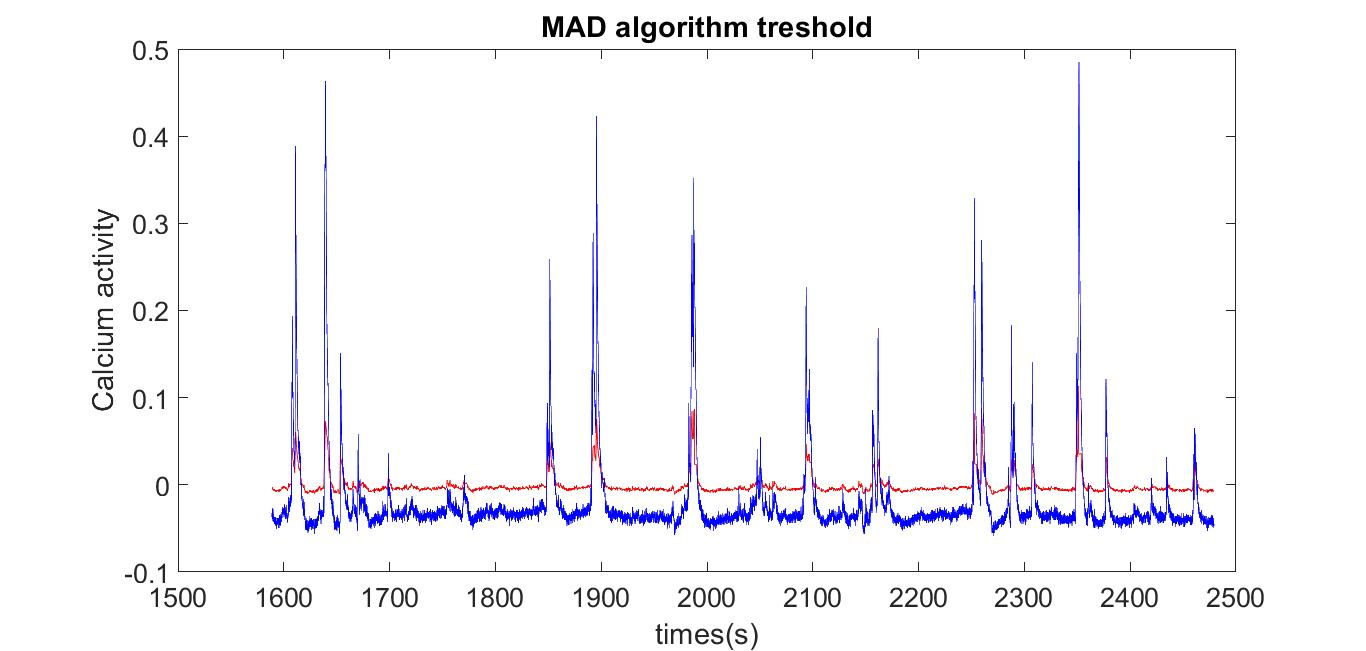
\includegraphics[scale=.30]{MAD.jpg} 
	\end{center}  
	
	
\end{figure}

\end{frame}

\begin{frame}
\frametitle{Characteristic time for an event}

Choosen time window: $ \tau = 250  ms$ \vspace{1.4 cm}

\begin{figure}[H]
	\begin{center}
		\hspace*{-1.3cm}
		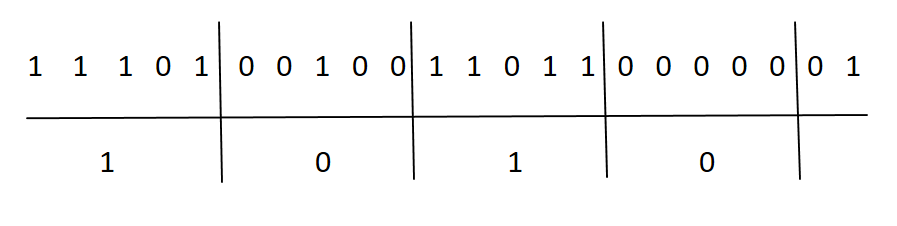
\includegraphics[scale=.45]{intervals.png} 
	\end{center}  
	
	
\end{figure}

\end{frame}

\begin{frame}
\frametitle{Peak correlation index}

$$ i_{AB} = \frac{N_{AB} T}{N_A N_B dT} $$ \vspace{0.5 cm}


$T = $ overall signal time window \\ \vspace{0.5 cm}

$dT = $ synchronization time window \\ \vspace{0.5 cm}

$N_A = $ Number of peaks in signal A \\ \vspace{0.5 cm}

$N_B = $ Number of peaks in signal B \\ \vspace{0.5 cm}



$N_{AB} = \sum_{i=1}^{N_A} \sum_{j=1}^{N_B} I_{[-dT,dT]}(|a_i - b_j|) $

\end{frame}

\begin{frame}
\frametitle{Distance analysis}

Linear fit: $ R^2 = 0.024$ 

\begin{figure}[H]
	\begin{center}
		\hspace*{-1.3cm}
		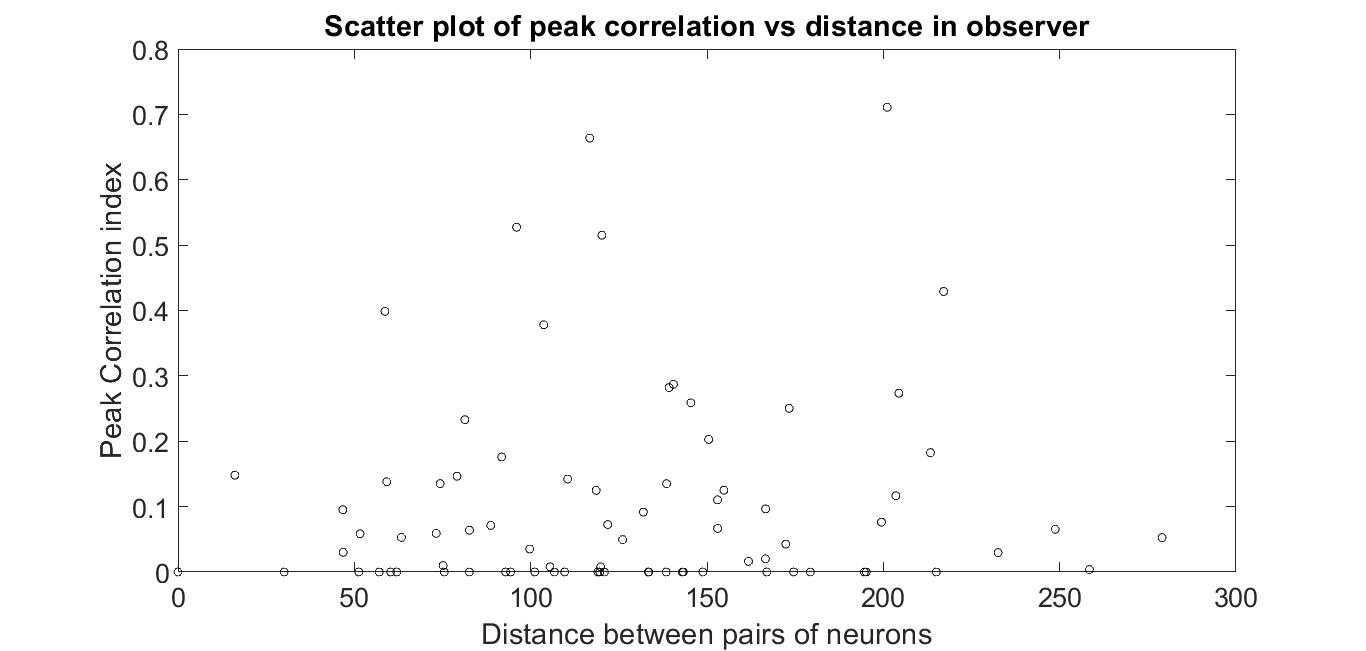
\includegraphics[scale=.30]{distance.jpg} 
	\end{center}  
	
	
\end{figure}

\end{frame}

\begin{frame}
\frametitle{Peak correlation in single mouse (I dataset)}


\begin{figure}[H]
	\begin{center}
		\hspace*{-1.3cm}
		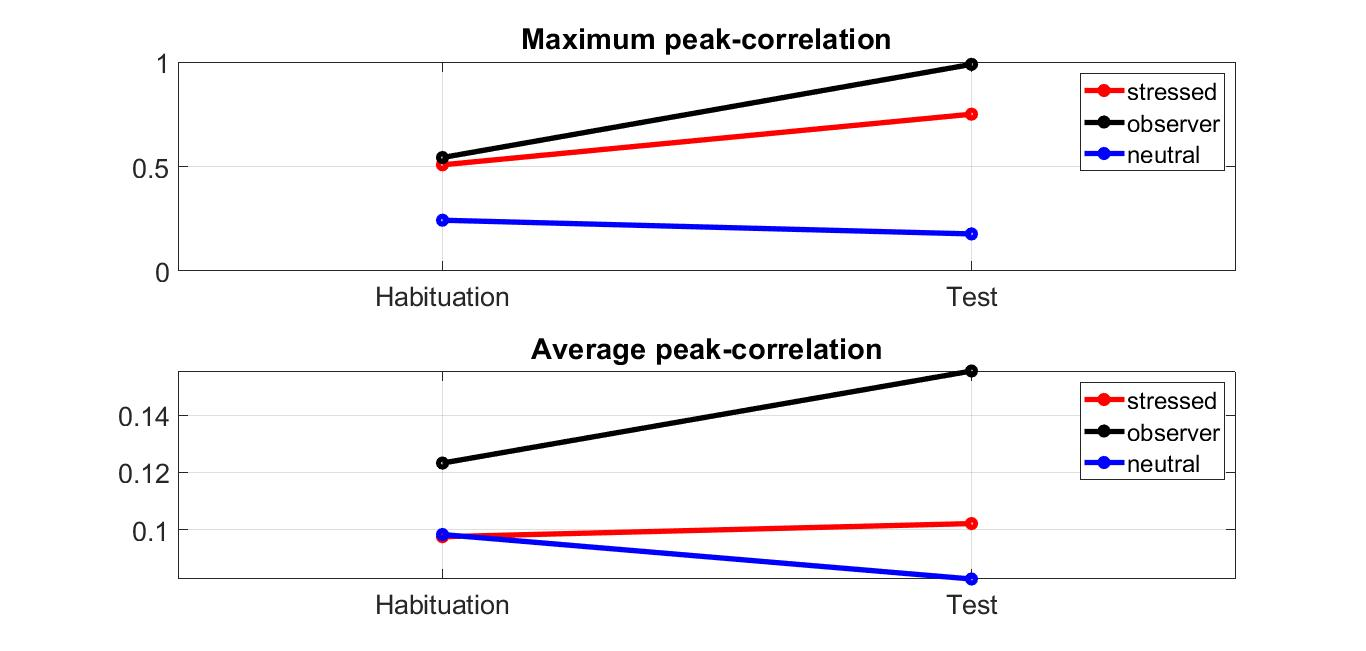
\includegraphics[scale=.30]{peak_corr.jpg} 
	\end{center}  
	
	
\end{figure}

\end{frame}

\begin{frame}
\frametitle{Peak correlation in single mouse (II dataset)}


\begin{figure}[H]
	\begin{center}
		\hspace*{-1.3cm}
		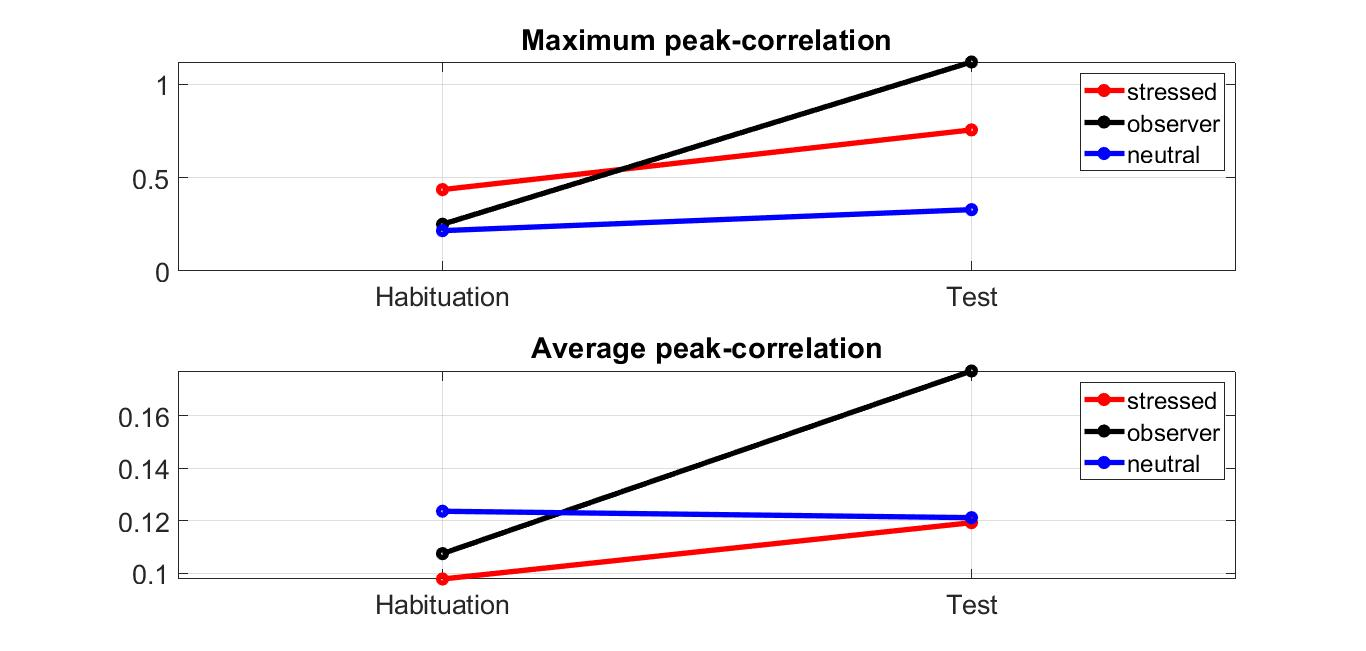
\includegraphics[scale=.30]{peak_corr2.jpg} 
	\end{center}  
	
	
\end{figure}

\end{frame}

\begin{frame}
\frametitle{Peak correlation in single mouse (III dataset)}


\begin{figure}[H]
	\begin{center}
		\hspace*{-1.3cm}
		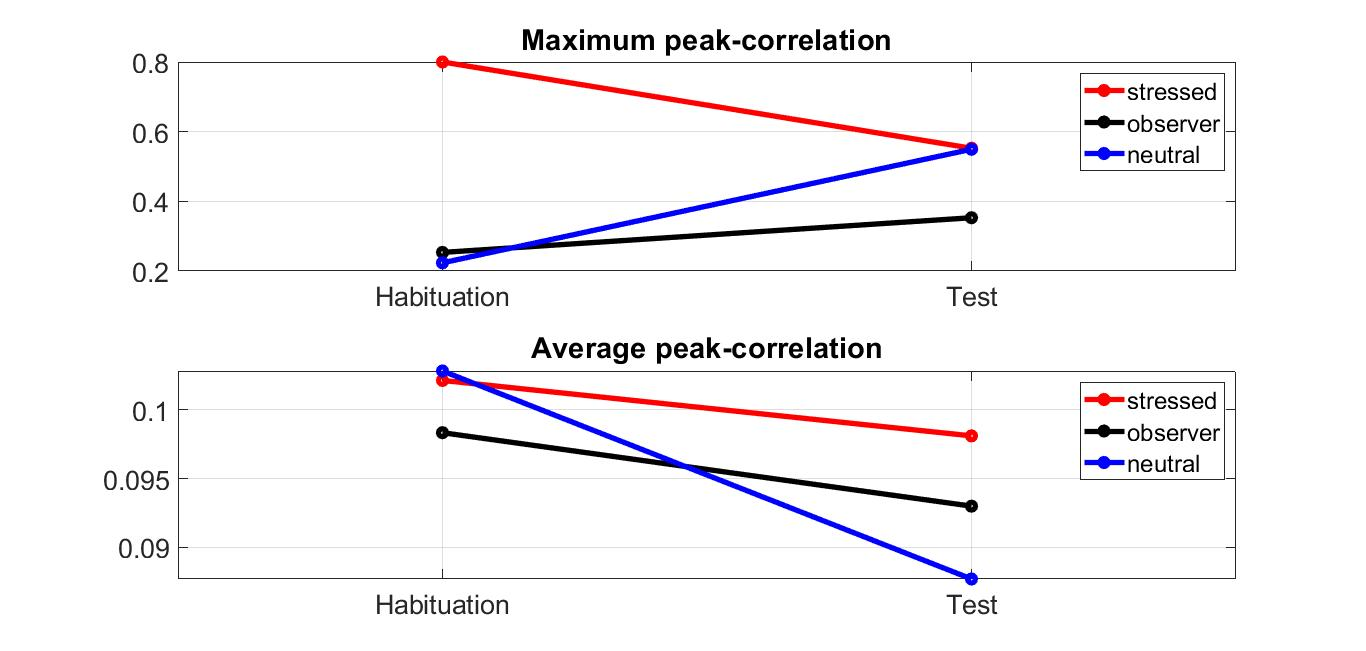
\includegraphics[scale=.30]{peak_corr3.jpg} 
	\end{center}  
	
	
\end{figure}

\end{frame}

\begin{frame}
\frametitle{Peak correlation in single mouse (IV dataset)}


\begin{figure}[H]
	\begin{center}
		\hspace*{-1.3cm}
		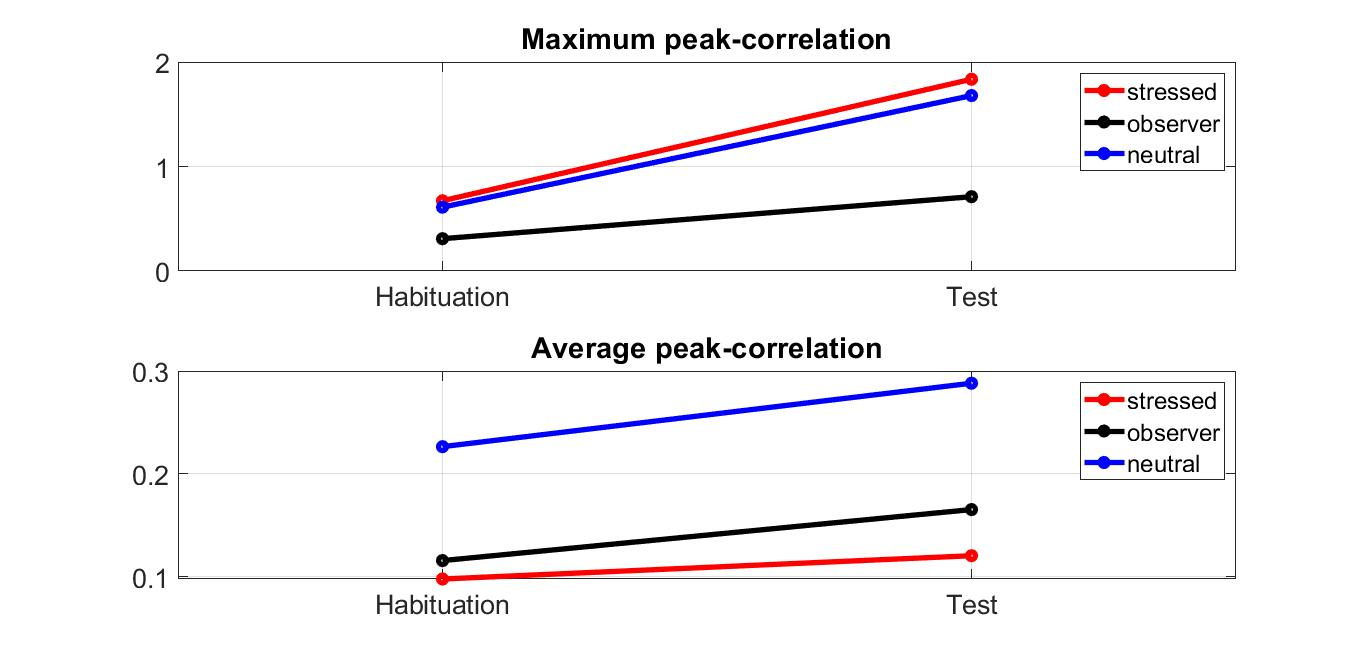
\includegraphics[scale=.30]{peak_corr4.jpg} 
	\end{center}  
	
	
\end{figure}

\end{frame}

\begin{frame}
\frametitle{Peak synchronization between mice (I dataset)}


\begin{figure}[H]
	\begin{center}
		\hspace*{-1.3cm}
		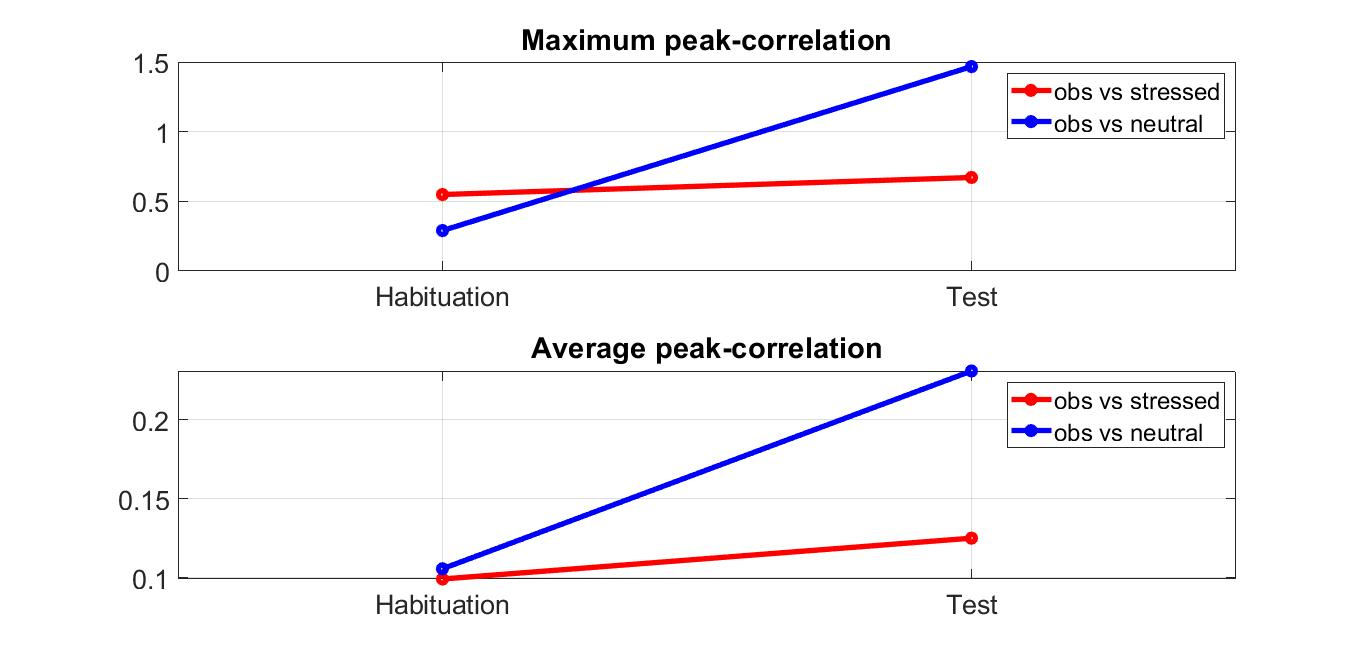
\includegraphics[scale=.30]{peak_synch.jpg} 
	\end{center}  
	
	
\end{figure}

\end{frame}

\begin{frame}
\frametitle{Peak synchronization between mice (II dataset)}


\begin{figure}[H]
	\begin{center}
		\hspace*{-1.3cm}
		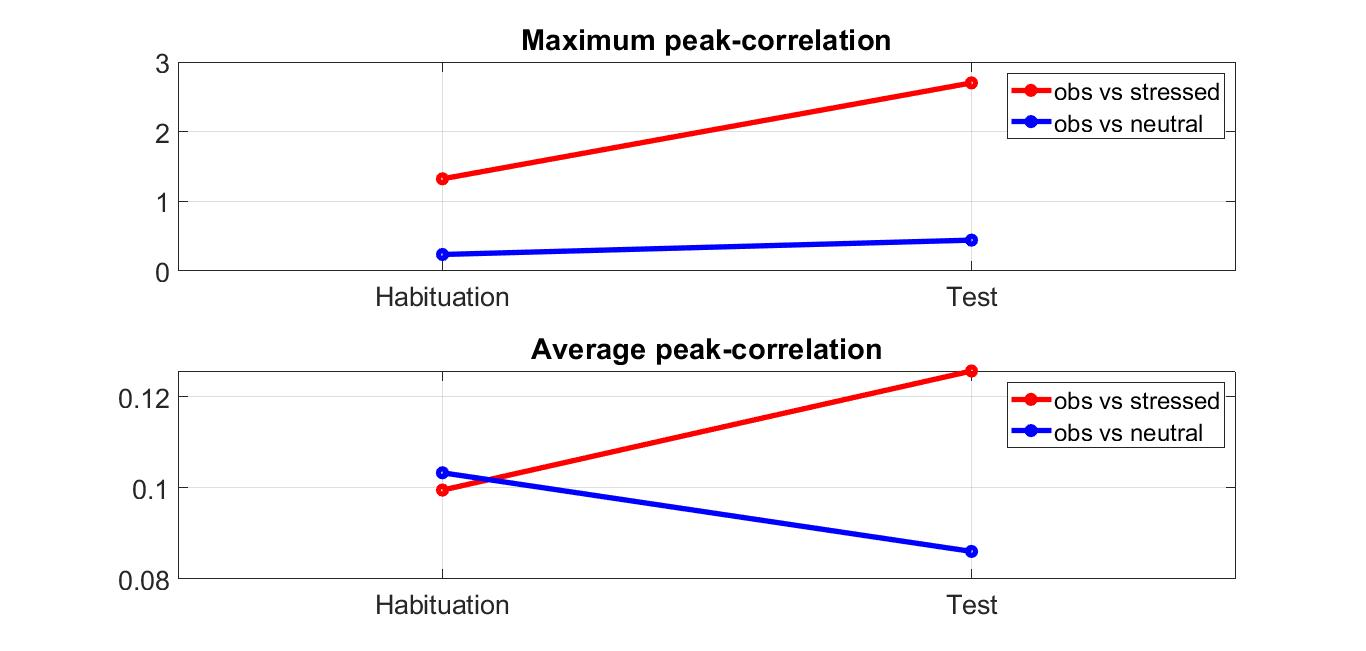
\includegraphics[scale=.30]{peak_synch2.jpg} 
	\end{center}  
	
	
\end{figure}

\end{frame}

\begin{frame}
\frametitle{Peak synchronization between mice (III dataset)}


\begin{figure}[H]
	\begin{center}
		\hspace*{-1.3cm}
		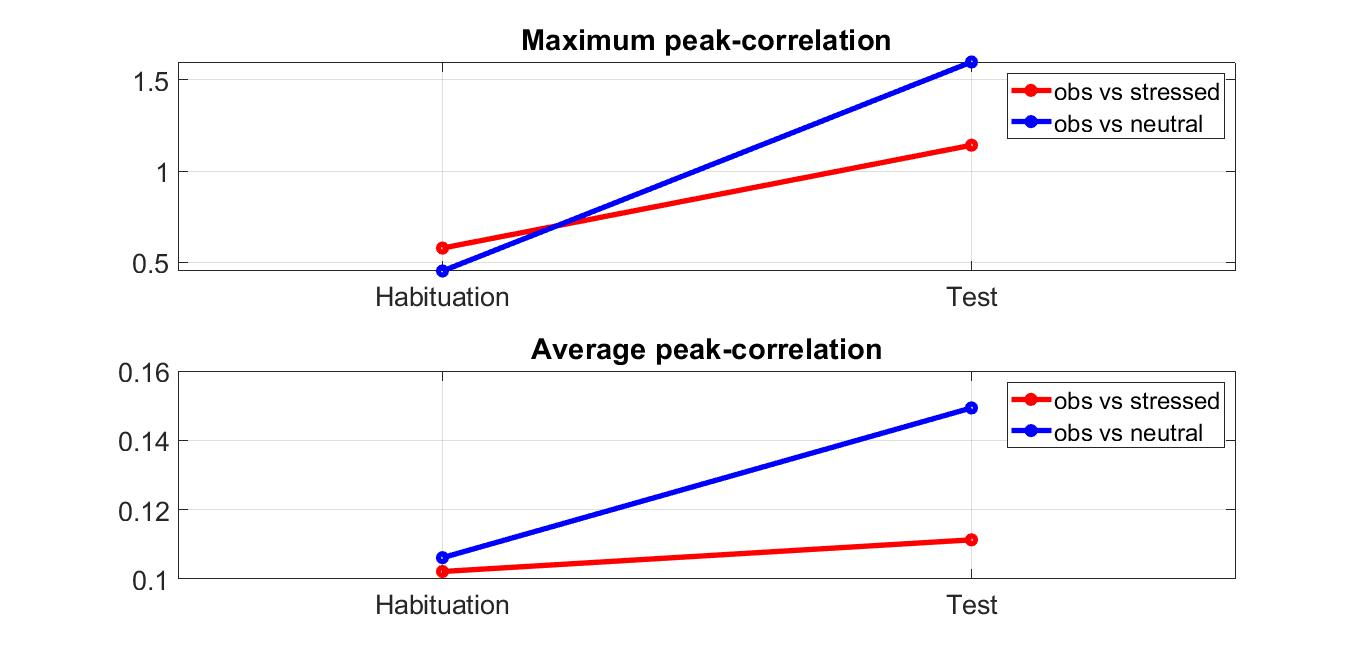
\includegraphics[scale=.30]{peak_synch3.jpg} 
	\end{center}  
	
	
\end{figure}

\end{frame}

\begin{frame}
\frametitle{Peak synchronization between mice (IV dataset)}


\begin{figure}[H]
	\begin{center}
		\hspace*{-1.3cm}
		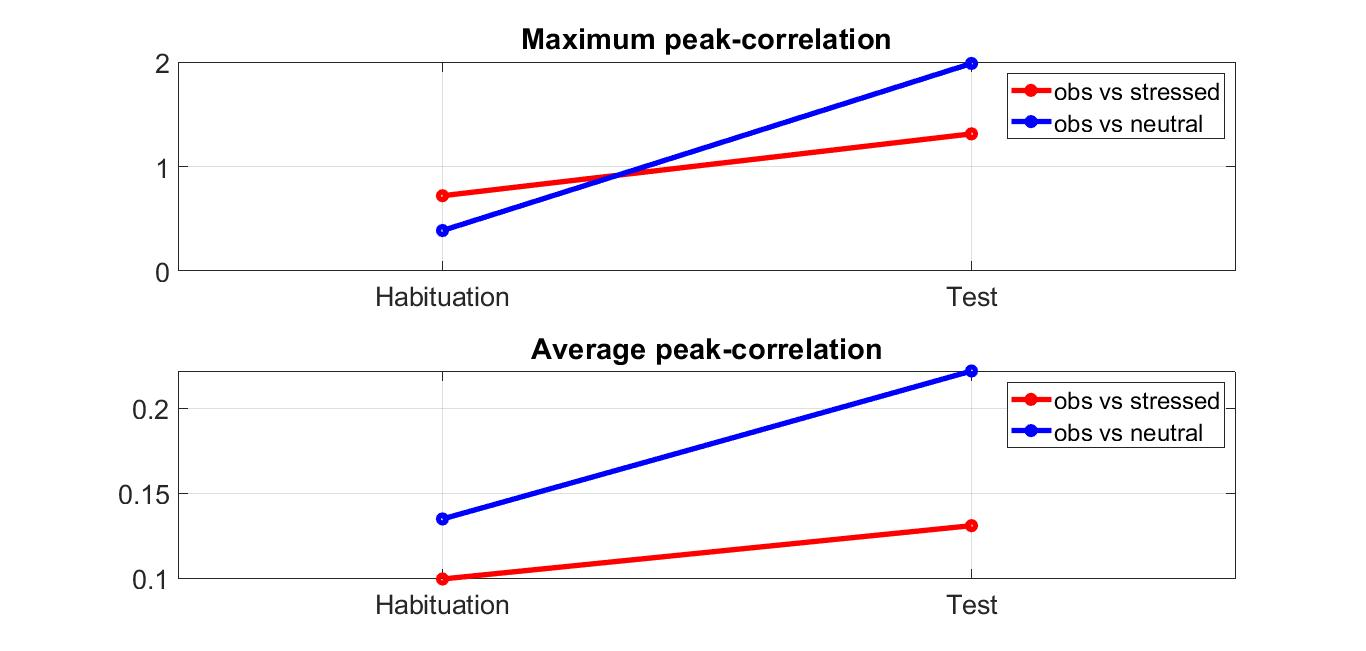
\includegraphics[scale=.30]{peak_synch4.jpg} 
	\end{center}  
	
	
\end{figure}

\end{frame}


\end{document}

\begin{frame}
\frametitle{}
\end{frame}